\begin{figure}[htbp]
    \centering
    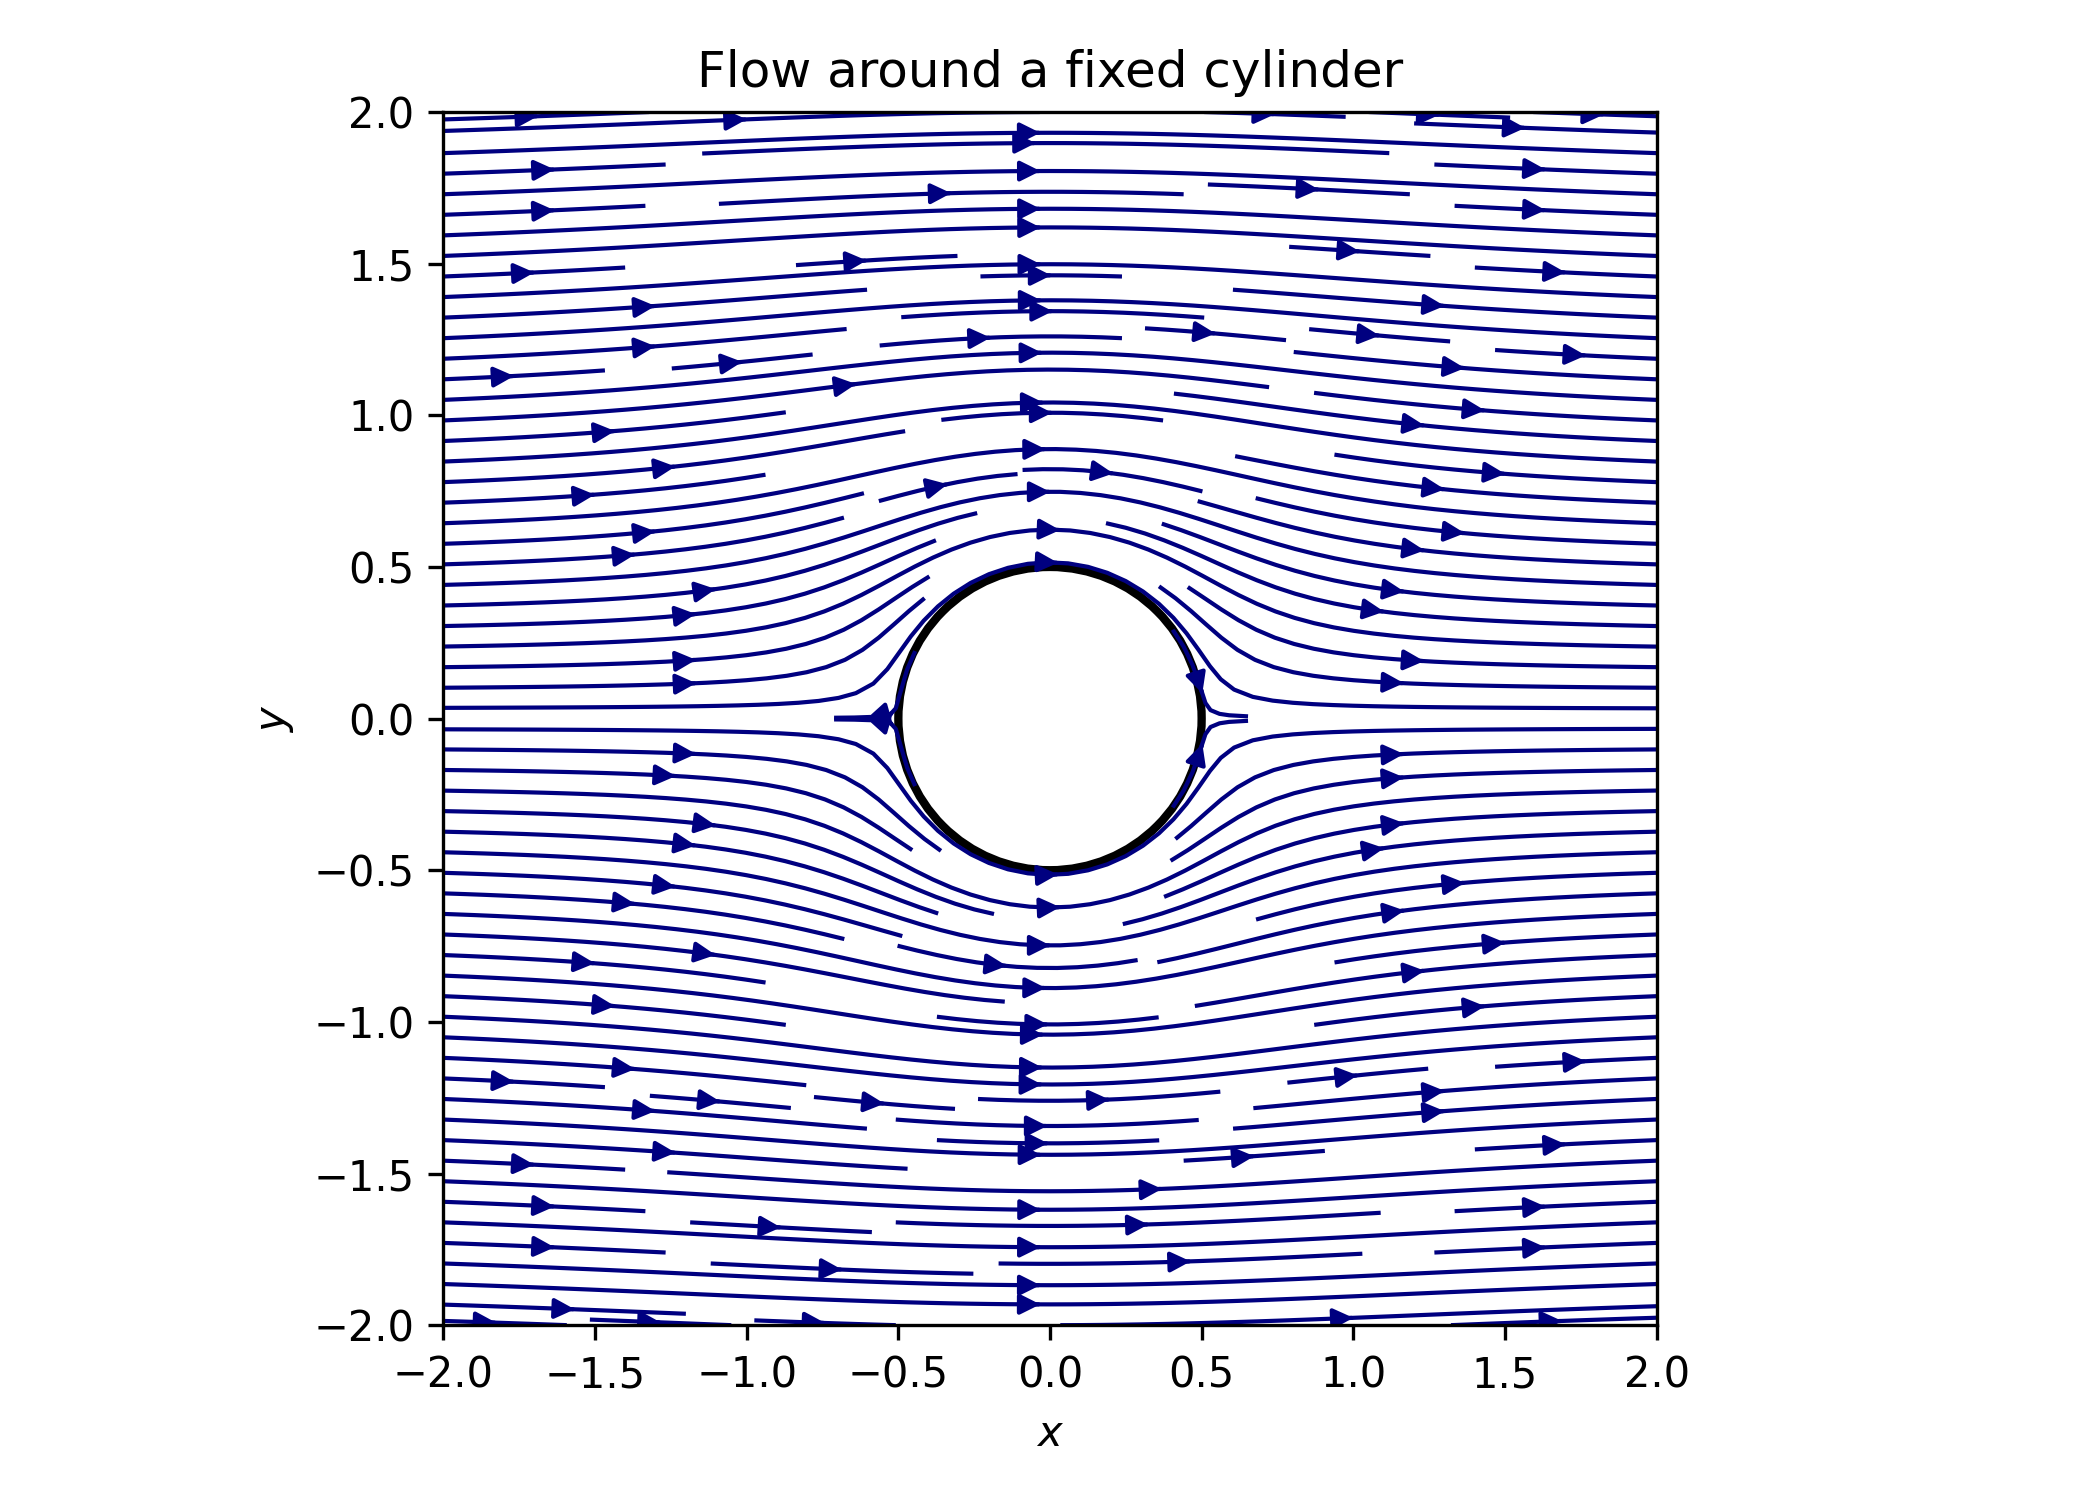
\includegraphics[width=0.85\textwidth]{../02_cylinder_flow}
    \caption{Visualization of flow around a fixed cylinder as an analogy for æther flow around a stable vortex in the æther model. The uniform background flow is locally distorted by the presence of the vortex structure. This classical potential flow profile forms the basis for later interpretations of æther interactions in the model.}
    \label{fig:cylinderflow}
\end{figure}

\section{Introduction}
In a modern revival of Lord Kelvin's vortex-atom hypothesis of 1867~\cite{Kelvin1867-vortex}, we consider an absolute Euclidean space filled with a superfluid æther. This contemporary æther interpretation builds upon and extends historical frameworks such as the Lorentz–Poincaré ether theory, which introduced absolute frames and mechanical interpretations of relativistic phenomena. Unlike those early theories, however, the present model explicitly incorporates modern fluid dynamics, topological vortex theory, and quantum mechanical structure, distinguishing it in both conceptual rigor and empirical relevance. Thus, it maintains historical continuity while offering a modernized and experimentally verifiable framework.

In this model, elementary particles are represented as stable vortex knots or nodes embedded in the æther, and \emph{time} is defined by the intrinsic angular rotation of their vortex cores. The challenge is to derive \emph{time dilation} laws—analogous to those in special and general relativity (SR and GR)—using ætheric parameters such as constant density, circulation, and Planck-scale time, rather than invoking 4D spacetime curvature. We require that any such formulation reproduces known relativistic effects—for example, the slowing of clocks near massive bodies (gravitational redshift) or at high relative velocities (special-relativistic dilation)—despite operating in a flat, 3-dimensional absolute background. In other words, the \emph{eddy dynamics} of the æther—as illustrated in Figure~\ref{fig:cylinderflow}—must replicate the curvature-induced metric effects of general relativity with high fidelity.

Historically significant experiments such as Michelson–Morley (1887), Pound–Rebka (1959), and Gravity Probe A (1976) offer indirect yet consistent support for an æther-based interpretation of relativistic phenomena. The Michelson–Morley experiment placed stringent constraints on uniform æther drift, while the Pound–Rebka experiment confirmed the gravitational redshift predicted by Einstein. Gravity Probe A further verified gravitational time dilation with high precision. These observations can be interpreted naturally within the vortex æther framework presented here, providing empirical coherence across historical and modern domains.

This paper develops a mathematically rigorous model for time dilation based on vortex rotation dynamics in an incompressible, inviscid superfluid æther. We begin by formalizing the fundamental postulates of the æther model and defining how the rotation of a microscopic vortex constitutes a physical clock. We then derive two classes of time dilation laws: one for motion through the æther (analogous to SR), and one for vorticity-induced inflows around mass (analogous to GR). We demonstrate that these results quantitatively reproduce standard relativistic predictions—such as gravitational redshift and orbital clock effects—while replacing spacetime curvature with structured æther flows and vortex angular velocity fields as the origin of time dilation.
